\chapter{Einleitung}
%Begonnen werden soll mit einer Einleitung zum Thema: z.B. Hintergrund und Ziel
%(was, warum).
In vielen Computerspielen ist eine Funktion von N�ten um Einheiten und Charaktere ans Ziel zu f�hren. Egal in welchen Genre, wenn sich der Computer in einer simulierten Umgebung effizient zurecht finden soll, wird ein Wegfindealgorithmus ben�tigt. Um Umwege und unnat�rlich wirkendes Verhalten zu vermeiden, bietet sich ein heuristischer, Graphen basierter Algorithmus an.
Dieser hat sich als effizienteste L�sung f�r Wegfindeprobleme erwiesen.\\
Nicht nur in Civilization, wo die Funktionsweise dem Spieler als ein Zentrales Spielelement bewusst wird, finden solche Algorithmen Verwendung. Auch Genres scheinbar abseits taktischer Tiefe, wie Beispielsweise MMORPGS oder Shootern w�ren ohne dieselben nicht realisierbar.\\

%In vielen Jahren der Spieleentwicklung hat sich A*(A-Stern) als der Effizienteste seiner Art herauskristallisiert.
Wegen seiner einfachen Implementierung und seines hohen Effizienzgrades hat sich A*(A-Stern) als Geeignetster seiner Art bew�hrt. Daher wird heute kaum noch auf andere L�sungen zur�ckgegriffen um entsprechende Probleme zu bew�ltigen. In so fern wird sich diese Arbeit mit den Eigenschaften und der Umsetzung in Programmen von A* befassen.

\chapter {Dijkstra}
Dijkstra bildet die Grundlage zu A*. Er wurde vom gleichnamigen Professor im Jahr 1959 in einem Lehrbuch erl�utert.\footnote{\cite{EWD:NumerMath59}} Es ist der �blichste Algorithmus, der sowohl f�r Netwerkrouting eingesetzt wird, als auch f�r Kartennavigationsger�te.\footnote{\cite{tanenbaum:CN}} \\

\section {Funktionsweise}
Der Dijkstra-Algorithmus bedient sich unterschiedlicher Funktionen um die k�rzeste Route zu finden:
\begin{itemize}
	\item Die Kosten des ersten Knotens betragen 0.
	\item Sonstige Knotenkosten akkumulieren sich aus den Kosten der Vorg�ngerknoten.
	\item Die Unbekannten ausgenommen, hat jeder Knoten ein Vorg�nger, der die bisher k�rzeste Verbindung zum ersten Knoten darstellt.
	\item fertig untersuchte Knoten werden ignoriert
		
\end{itemize}

 Die allgemeine iterative Vorgehensweise l�uft folgenderma�en ab:
\begin{enumerate}
	\item Die Knoten werden in 3 Listen sortiert
	\begin{itemize}
		\item unbekannte Knoten
		\item zu untersuchende Knoten
		\item fertig untersuchte Knoten
	\end{itemize}
	\item Am Anfang ist der Startknoten als "zu untersuchend" markiert, alle Anderen sind unbekannt.
	\item Aus der Liste der zu untersuchenden Knoten wird nun jener erw�hlt, welcher am wenigsten Kosten verursacht. \item Dieser wird nun in die Liste der fertig untersuchten Knoten verschoben.
	\begin{itemize}
		\item War dies der Zielknoten, so hat man als Ergebnis den Weg vom Anfang bis zum Ziel f�hrt.
		\item Wenn nicht, so werden die unbekannten, direkt verbundenen Knoten in die Liste der zu Untersuchenden gesetzt. Dabei werden die Kosten der Knoten ermittelt.\\ 
		Es gilt:\\
		$Weg+Kante= Knotenkosten$
		\\
		Falls f�r den Knoten schon einmal Kosten ermittelt wurden, so wird der niedrigste Betrag �bernommen.
	\end{itemize}
\end{enumerate}
Schritte 2 und 3 werden wiederholt bis die Liste der zu Untersuchenden Knoten leer ist. Bei einem erfolgreichen Ablauf, kann vom Ziel bis zum Startknoten der k�rzeste Weg verfolgt werden.\\
Falls das Ziel nicht erreicht wurde, gibt es keinen Weg �ber die angegebenen Knoten.
\begin{figure} %[hbtp]
	
	\centering
		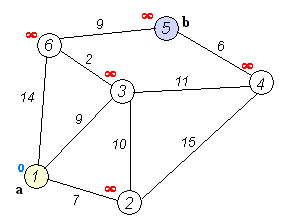
\includegraphics[width=0.25\textwidth]{images/Dijkstra-Beispiel/0.png}
	\caption{Start}
	\label{Schritt1}
\end{figure}

-A*
-D*?
